%----------------------------------------------------------------------
\begin{frame}[c]{Final Project}
    \begin{itemize}
        \item Hands-on experience on topics of the course
        \item Part of the oral exam
        \item Your evaluation builds the basis for discussion
        \item \alert{Scientifically analyze the important aspects\\ \& characteristics of your approach}
    \end{itemize}
\end{frame}
%----------------------------------------------------------------------
%----------------------------------------------------------------------
\begin{frame}[c]{General Information}
\begin{itemize}
    \item You will get access to your own bitbucket repository
    \item Submit your final code and any plots or tables of your results
    \item Deadline: 18.03 (23:59 GMT+1)
    \item 15 minutes discussion of your results in the exam
    \item You are allowed at most 5 slides
        \begin{itemize}
            \item Motivation
            \item Approach (2-3)
            \item Results (2-3)
        \end{itemize}
\end{itemize}
\end{frame}
%----------------------------------------------------------------------
%----------------------------------------------------------------------
\begin{frame}[c]{Task}
\begin{itemize}
    \item Your task is to optimize/analyze the performance of \textit{lpg}
    \pause
    \item How you optimize the performance of lpg is up to you
    \pause
    \begin{itemize}
     	\item Decide carefully whether selection (PIAC; next week) or configuration\\ is the correct approach
     	\item If you pick the right approach, you have to invest roughly 4h\\ (without validation \& further analysis) 
    \end{itemize}
    \pause
    \item The final performance is to be measured in terms of CPU-time
    \item lpg should run no longer than 100 seconds on an instance
    \pause
    \item We will provide machines to make all results comparable
\end{itemize}
\end{frame}
%----------------------------------------------------------------------
%----------------------------------------------------------------------
\begin{frame}[c]{Task}
We will provide you with:\\
\begin{itemize}
    \item An instance set consisting of AI planning instances.
    \pause
    \item A file listing all training and test instances.
    \pause
    \item The binary of \textit{lpg}
    \item A file detailing it's parameter configuration space (params.pcs).
    \pause
    \item A wrapper that is capable of calling \textit{lpg} and parsing its output.
    \pause
    \item A csv file consisting of instance features for all training and test instances.
    \pause
    \item We provide three machines (each equipped with two Intel Xeon E5-2650v2 8-core CPUs, 20 MB L2 cache and 64 GB of (shared) RAM per machine, running Ubuntu 14.04 LTS 64 bit) which you can work remotely on and test / evaluate your implementation.
\end{itemize}
\end{frame}
%----------------------------------------------------------------------
%----------------------------------------------------------------------
\begin{frame}[c]{Task}
\begin{itemize}
    \item lpg has 67 parameters (mixture of continuous and categoricals)
    \item You are given 655 Training and 67 test instances
\end{itemize}
\begin{figure}
    \centering
    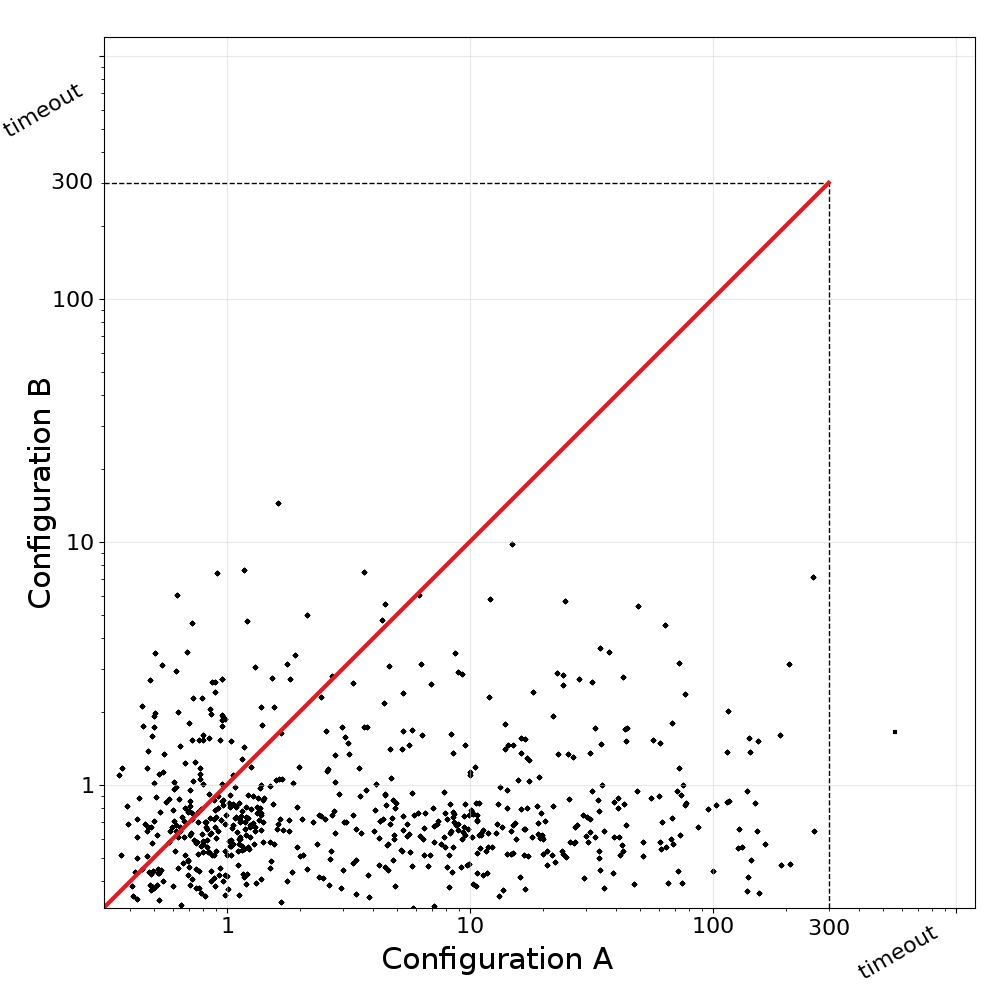
\includegraphics[width=.5\textwidth]{exercises/scattertrain}
    \caption{Example results on training data}
\end{figure}
\end{frame}
%----------------------------------------------------------------------
%----------------------------------------------------------------------
\begin{frame}[c]{Possible parts of solving the task}
\begin{itemize}
    \item Measure the default performance of \textit{lpg}
    \pause
    \item Plot the performance
    \pause
    \item Guess whether it is a heterogeneous or an homogeneous instance set, to apply PIAC or AC
    \pause
    \item Apply algorithm configuration to determine a well-performing configuration
    \pause
    \item Determine the importance of \textit{lpg}'s parameters
    \pause
    \item Optimize an algorithm schedule of configurations
    \pause
    \item Apply algorithm selection to select well-performing configurations
    \pause 
    \item Plot the performance of the optimized vs the default configuration
    \pause
    \item Report the performance (PAR1, PAR10, number of timeouts)
    \pause
    \item Construct an EPM from observed data and predict well performing configurations
\end{itemize}
\end{frame}
%----------------------------------------------------------------------
%----------------------------------------------------------------------